%!TEX root = ../../report.tex
\clearpage
\subsection{Deployment View}
This subsection outlines the physical arrangement of the nodes in a distributed system, the artifacts that are stored on each node, and the components and other elements that the artifacts implement \cite{ibmdeployment}. Communication paths and deploy relationships model the connections in the system.

\subsubsection{Deployment Diagram}
Figure \ref{fig:deployment-diagram} shows the deployment diagram of the \gls{SFM}. The diagram contains several components such as, sensors, \gls{UAV}, analytics clusters, and database clusters. Main communication between components are done using TCP/IP. All hardware decision are based on chapter 6.
	
% \clearpage

\begin{landscape}
	\begin{figure}[H]
		\centering
		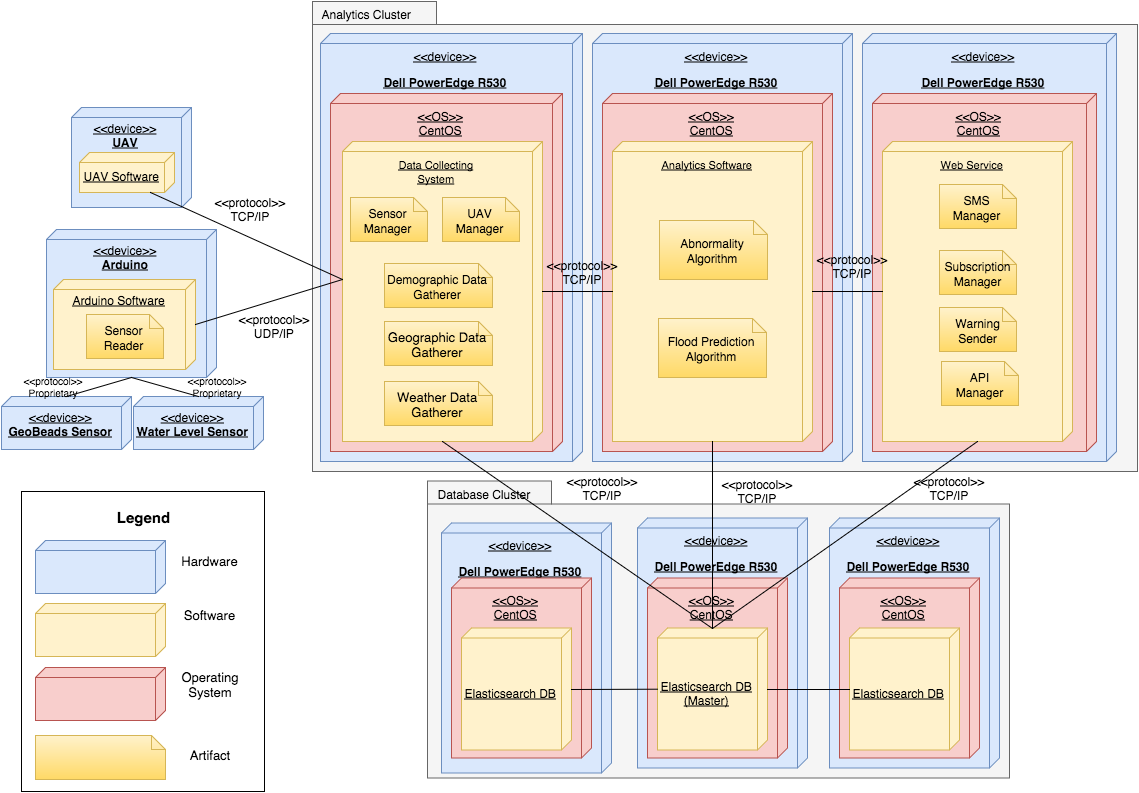
\includegraphics[keepaspectratio=true,width=1.0\textwidth]{{\viewimages/deployment-view}.png}
		\caption{Deployment diagram}
		\label{fig:deployment-diagram}
	\end{figure}
\end{landscape}

% \clearpage

The deployment diagram, depicted in figure \ref{fig:deployment-diagram}, is developed based on \cite{ibmdeployment}. The block with blue color represents hardware components. The red and yellow represent operating system and the SFM developed software. Some artifacts are put inside the software block. Deployment view can be categorized into three main components, which are sensing components, main analytics cluster, and database cluster.

\subsubsection*{Sensing Components}
This portion of the \gls{SFM} is responsible for gathering required data and sending the data to Data Collection System. The \gls{SFM} will utilize two kind of sensor, water level sensor and GeoBeads sensor. Water level sensor is required to measure the water condition of dykes or water ways, while GeoBeads sensor is used to measure the dykes condition. Both kind of the sensor does not have any software part in it as it is merely electronic component that senses the condition of the surroundings. Both of the sensor will be directly connected to Arduino Uno Ethernet. Arduino will pack the data gathered from sensors and periodically send it to the Data Collecting System.

Furthermore, \gls{UAV} will fly if it is necessary. \gls{UAV} will take certain pictures, which is impossible for human to take it, that will be useful for maintenance of the \gls{SFM} or fixing certain problem.

\subsubsection*{Main Analytics Clusters}
Main analytics cluster is responsible for gathering data and storing it to the database, detecting possible faulty sensors, and analyzing the gathered data to predict imminent flood. The main analytics cluster consist of three main components: data collecting system, analytics cluster, and web service that is open to public.

The \gls{SFM} will run three data centers to maintain the key drivers of the system. Two of them will be located inside the Netherlands and one will be located abroad. However, figure \ref{fig:deployment-diagram} only shows one of them for the sake of simplicity.

\subsubsection*{Database Cluster}
This component will store the data coming from sensors and \gls{UAV}. The \gls{SFM} will not store any weather data because the data is always available in the weather provider, thus there is no need to store the data. The \gls{SFM} will run Elasticsearch database because it is suitable for storing data that the \gls{SFM} will have.

\subsubsection{Artifacts}
Figure \ref{fig:deployment-diagram} contains several artifacts that are derived from \autoref{fig:elaborated-model}, \autoref{fig:layers}, \autoref{fig:logical}, \autoref{fig:component}, and \autoref{fig:package-diagram}. Elaboration of the artifacts will also be categorized into two main components: sensing components and main analytics cluster.

\subsubsection*{Sensing Components}
\begin{table}[H]
	\begin{tabular}{L{0.2\textwidth} L{0.6\textwidth}}
		\textbf{Artifact} & \textbf{Description}                                                                           \\ \toprule
		Sensor Reader     & Sensor reader is responsible for packing the data gathered from sensor to be ready to be sent. \\ \bottomrule
	\end{tabular}
	\caption{Artifact for sensing component}
	\label{table:sensing-artifacts}
\end{table}

\subsubsection*{Main Analytics Clusters}
% \begin{longtabletable}[H]
\begin{longtable}{L{0.2\textwidth} L{0.6\textwidth}}
	\centering
	\textbf{Artifact}          & \textbf{Description}                                                                              \\ \toprule
	Sensor Manager             & Sensor manager is responsible for managing input 									coming from multiple sensors (Arduino). \\ \midrule
	\gls{UAV} Manager          & \gls{UAV} manager is responsible for handling incoming 							 data from \gls{UAV}s.              \\ \midrule
	Demographic Data Gatherer  & This is responsible for getting data from demographic 							data provider.                       \\ \midrule
	Geographic Data Gatherer   & This is responsible for getting data from geographic 								data provider.                       \\ \midrule
	Weather Data Gatherer      & This is responsible for getting data from weather data 							 provider.                          \\ \midrule
	Abnormality Algorithm      & Abnormality algorithm is responsible for detecting 								faulty sensors.                        \\ \midrule
	Flood Prediction Algorithm & This is the main part of algorithm, which will detect 							imminent flood.                      \\ \midrule
	SMS manager                & SMS manager is responsible for handling outgoing SMS 								to certain users.                    \\ \midrule
	Subscription Manager       & Subscription manager is responsible for managing 									subscription of citizens/users.         \\ \midrule
	Warning Sender             & Warning sender is responsible for sending warnings to 							Safety region.                       \\ \midrule
	API Manager                & This is responsible for managing outgoing API to third 							 party developers.                  \\ \bottomrule
	\caption{Artifact for main analytics cluster}
	\label{table:main-analytics-artifacts}
\end{longtable}

% \end{longtable}
